%%  Assignment 4 for CSC263H1, Fall 2015,
%%  at the University of Toronto.
%%
%%  Copyright (c) 2014 Toniann Pitassi <toni@cs.utoronto.ca>
%%  last updated at 09:02 (EDT) on Mon  9 Mar 2015
%%
%%  CC BY-SA 4.0
%%  This work (the current file named 'A2handout.tex') is licensed under
%%  the Creative Commons Attribution-ShareAlike 4.0 International License.
%%  To view a copy of this license, visit
%%      http://creativecommons.org/licenses/by-sa/4.0/
%%  or send a letter to: Creative Commons, 444 Castro Street, Suite 900,
%%  Mountain View, California, 94041, USA.
%%  This is a human-readable summary of (and not a substitute for) the
%%  license.
%%  You are free to:
%%      Share -- copy and redistribute the material in any medium or format
%%      Adapt -- remix, transform, and build upon the material for any
%%          purpose, even commercially.
%%      The licensor cannot revoke these freedoms as long as you follow the
%%          license terms.
%%  Under the following terms:
%%      Attribution -- You must give appropriate credit, provide a link to
%%          the license, and indicate if changes were made. You may do so in
%%          any reasonable manner, but not in any way that suggests the
%%          licensor endorses you or your use.
%%      ShareAlike -- If you remix, transform, or build upon the material,
%%          you must distribute your contributions under the same license as
%%          the original.
%%      No additional restrictions -- You may not apply legal terms or
%%          technological measures that legally restrict others from doing
%%          anything the license permits.
%%  Notices:
%%      You do not have to comply with the license for elements of the
%%      material in the public domain or where your use is permitted by an
%%      applicable exception or limitation.
%%      No warranties are given. The license may not give you all of the
%%      permissions necessary for your intended use. For example, other
%%      rights such as publicity, privacy, or moral rights may limit how you
%%      use the material.

\RequirePackage[l2tabu,orthodox]{nag}  % warn about common LaTeX pitfalls
\RequirePackage[ascii]{inputenc}  % input is 7-bit ASCII
\RequirePackage{fixltx2e}  % fix LaTeX2e kernel bugs

\documentclass[11pt,twoside]{article}
\usepackage{color}
\usepackage{tikz}
\usepackage{calc}  % arithmetic in length parameters
\usepackage{enumitem}  % more control over list formatting
\usepackage{fancyhdr}  % simpler headers and footers
\usepackage[margin=1in]{geometry}  % page layout
\usepackage{lastpage}  % for last page number
\usepackage{relsize}  % easier font size changes
\usepackage[normalem]{ulem}  % smarter underlining
\usepackage{url}  % verb-like typesetting of URLs
%\usepackage{xfrac}  % nicer looking simple fractions for text and math
\usepackage{amsmath}
\usepackage{amssymb}

% Set up fonts.
\usepackage[T1]{fontenc}  % use true 8-bit fonts
\usepackage{slantsc}  % allow slanted small-caps
\usepackage{microtype}  % perform various font optimizations
% Version 1.2 (2015/02/08) of newpxtext messes up \textsl so skip it...
% Use Palatino-based monospace instead of kpfonts' default.
%\usepackage{newpxtext}
%\ttfamily
%\DeclareFontShape{T1}{\ttdefault}{m}{scsl}{<->ssub*\ttdefault/m/sc}{}
%\DeclareFontShape{T1}{\ttdefault}{b}{scsl}{<->ssub*\ttdefault/b/sc}{}
% "Kepler" fonts.
\usepackage[nott,notextcomp]{kpfonts}
% Use curvier Latin Modern brackets instead of kpfonts' glyphs.
\DeclareSymbolFont{lmsymb}     {OMS}{lmsy}{m}{n}
\DeclareSymbolFont{lmlargesymb}{OMX}{lmex}{m}{n}
\DeclareMathDelimiter{\rbrace}{\mathclose}{lmsymb}{"67}{lmlargesymb}{"09}
\DeclareMathDelimiter{\lbrace}{\mathopen}{lmsymb}{"66}{lmlargesymb}{"08}

% Page layout: stretch text to fill up page.
\addtolength\footskip{.25\headheight}
\flushbottom

% Common macros.
\input{macros-263}

% Headings.
\pagestyle{fancy}
\let\headrule\empty
\let\footrule\empty
\lhead{CSC\,263\,H1}
\chead{\large\scshape Assignment \#\,4}
\rhead{\scshape Fall 2015}
\lfoot{\scshape Dept.\@ of Computer Science, University of Toronto,
       St.~George Campus}
\cfoot{}
\rfoot{\scshape page \thepage\space of \pageref{LastPage}}


\begin{document}

\noindent
\strong{Worth:}  8\%
\hfill
\strong{Due:}  By 5:59pm on Tuesday 17 November\\[2ex]
\strong
   {Remember to write
    the \emph{full name} and \emph{student number}
    of \emph{every group member}
    prominently on your submission.}

\medskip

\noindent
\rule{\textwidth}{.5pt}\\[1ex]
\begingroup\slshape
    Please read and understand the policy on Collaboration
    given on the Course Information Sheet.
    Then, to protect yourself,
    list on the front of your submission
    \strong{every} source of information
    you used to complete this homework
    (other than your own lecture and tutorial notes).
    For example, indicate clearly
    the \strong{name} of every student from another group
    with whom you had discussions,
    the \strong{title and sections} of every textbook you consulted
    (including the course textbook),
    the \strong{source} of every web document you used
    (including documents from the course webpage),
    \etc.\par
        For each question, please write up detailed answers carefully.
    Make sure that you use notation and terminology correctly, and
    that you explain and justify what you are doing.
    Marks \strong{will} be deducted
    for incorrect or ambiguous use of notation and terminology, and
    for making incorrect, unjustified, ambiguous, or vague claims
    in your solutions.
\endgroup\\
\rule{\textwidth}{.5pt}
% If you use this file as a template for your solution, please remove
% (or comment out) the block above!

\begin{enumerate}[leftmargin=0pt]




\item
	In this question, we will use a graph algorithm to solve a problem
	in philosophy. 
	
	A \defn{paradox} is a group of statements that lead to a contradiction.
	For example, the following two statements form a famous paradox:
	\begin{verbatim}
		    1. Statement 2 is FALSE.
		    2. Statement 1 is TRUE.
	\end{verbatim}
	If we assume Statement 1 is \True, then Statement 2 is \False, which
	in turn means Statement 1 is \False. But if we assume Statement 1 is
	\False, then Statement 2 is \True, which in turn means Statement 1
	is \True. So Statement 1 is \True\ iff Statement 1 is \False, a blatant
	contradiction.

	Now, suppose you are given a group of $N$ statements, numbered from $1$
	to $N$. Each statement has the form: ``\code{Statement X is
	\True/\False},'' where \code{X} is a number between 1 and $N$. Your
	task is to figure out whether this group of statements forms a paradox.
	In particular, answer the following questions.
	\begin{enumerate}[label=(\alph*),topsep=\parsep]

	\item\label{graph}%
		Describe how to construct a graph to solve this problem. Be
		precise: state clearly what vertices your graph contains (and what
		each vertex represents) and what edges your graph contains (and what
		each edge represents).

	\item\label{condition}%
		Give a \strong{necessary and sufficient} condition for the $N$
		statements to form a paradox. Justify your answer.

	\item  How do you efficiently detect whether your graph from
		part~\ref{graph} satisfies your condition described in
		part~\ref{condition}? Describe your algorithm in concise (but
		precise) English.

	\item  Analyse the worst-case runtime of your algorithm.

	\end{enumerate}
	% answer for question 1
	\textcolor{red} {$Answer$}
	\begin{enumerate}[topsep=\parsep]
	% part a
	\item construct  graph $G(V,E)$
		\begin{itemize}[label = {}]
		\item \proc{V}: vertices set $V$ contains all $N$ statement. We order $V= \{v_1, v_2, v_3 ... v_N \}$ such that $v_i$ is a $i_{th}$ statement.
		\item  \proc{E}: There is edge $\vec{v_iv_j}$ with weight $1$ iff $i_{th}$ statement says $j_{th}$ statement
		is true.  There is edge $\vec{v_iv_j}$ with weight $-1$ iff $i_{th}$ statement says $j_{th}$ statement
		is false. 
		\end{itemize}
	% part b
	\item  
	Suppose $G(V,E)$ is the graph constructed from  N statements. let's define the truth assignment $\tau$ for this $G(V,E)$.
	\[ \tau:  V \rightarrow \{1, -1\}, \ \ \ where \ 1 \ stands \ for \ true \ and \ -1 \ for \ false\]
	\\
	Now lets define \proc{Stable} for a truth assignment $\tau$, a truth assignment $\tau$ is \proc{Stable} iff for any edge $\vec{v_iv_j} \in E$,
	 $\tau(v_i) \times \tau(v_j) = Weight(\vec{v_iv_j} )$. \\
	 \\
	 
	 Then let's define  random assignment $\Phi$,  random assignment $\Phi$ is a truth assignment which defined recursively as follows,
	 \begin{itemize}[label = {}]
	 \item Pick any vertex $a$ in graph $G(V,E)$ and assign $1$ to $a$.
	 \item for any node $v \in V$, $\forall v' \in Neighbours(A)$, 
	 \item \ \ \ \ \ \ \ \ if $Weight(\vec{vv'}) = 1$ or $Weight(\vec{v'v}) = 1$, then $\Phi(v') = \Phi(v)$;
	 \item  \ \ \ \ \ \ \ \ if $Weight(\vec{vv}') = -1$ or $Weight(\vec{v'v}) = -1$, then $\Phi(v') = -\Phi(v)$.
	 \item
	 \end{itemize} 
	 It's is obvious that random assignment $\Phi$ is stable, it can be derived from the definition of stable and random assignment.\\
	 Note: not all graph has a random assignment $\Phi$ (see following graphs).\\
	\begin{center}
            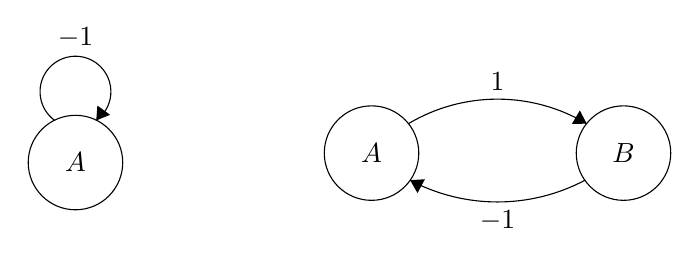
\begin{tikzpicture}[scale=0.2]
            \tikzstyle{every node}+=[inner sep=0pt]
            \draw [black] (24.1,-26.8) circle (3);
            \draw (24.1,-26.8) node {$A$};
            \draw [black] (42.9,-26.2) circle (3);
            \draw (42.9,-26.2) node {$A$};
            \draw [black] (58.9,-26.2) circle (3);
            \draw (58.9,-26.2) node {$B$};
            \draw [black] (45.237,-24.334) arc (120.82218:59.17782:11.052);
            \fill [black] (56.56,-24.33) -- (56.13,-23.49) -- (55.62,-24.35);
            \draw (50.9,-22.27) node [above] {$1$};
            \draw [black] (56.454,-27.923) arc (-62.08081:-117.91919:11.862);
            \fill [black] (45.35,-27.92) -- (45.82,-28.74) -- (46.29,-27.86);
            \draw (50.9,-29.8) node [below] {$-1$};
            \draw [black] (22.777,-24.12) arc (234:-54:2.25);
            \draw (24.1,-19.55) node [above] {$-1$};
            \fill [black] (25.42,-24.12) -- (26.3,-23.77) -- (25.49,-23.18);
            \end{tikzpicture}
           \end{center}
         For the left graph is we assign $1$ to A, then based on the weight of edge A should be assigned $-1$ hence, contradiction then no random assignment. Same for the right hand side graph.\\
         \\
	  $Claim:$ N statements do not form a paradox iff there exist a random assignment $\Phi$ for the corresponding graph $G(V,E)$. \\
	  \\ Here we only consider the case when $G(V, E)$ is connected. Since if $G(V, E)$ is not connected we can just check  random assignment $\Phi$  on each of its connected components. Therefore, it's sufficient to check just for connected graph.
	Proof
	\begin{itemize}
	\item ($\Leftarrow$) This direction is easy to prove, since if a graph has a stable random assignment $\Phi$ then just assign true and false to each statement
	corresponding with their truth value then clearly it's stable then no paradox.
	\item ($\Rightarrow$) Assume those N statements do not form a paradox, which means if we assign $true$ to any $a \in V$. We can get the truth assignment for all $a's$ neighbours(A). Basically, if $v \in Neighbours(A)$ then $v$ gets $true$ iff  $a_{th}$ statement says $v_{th}$  is true or $v_{th}$ statement says $a_{th}$ true and $v$ gets value $false$ iff  $a_{th}$ statement says $v_{th}$ is false or $v_{th}$ statement says $a_{th}$ false. Recursively we can get value of all vertices in $G(V,E)$, clearly if we assign $-1$ to false and $1$ to true this is exactly a random assignment $\Phi$ for $G(V,E)$.
	\end{itemize} 

	
	% part c
	\item  
	\begin{itemize}[label = {}]
		\item From $(b)$ we can get N statements  form a paradox iff there do not exist random assignment $\Phi$ for the corresponding graph $G(V,E)$, which means starts with any vertex $a$ with value $1$, we could not finish this assignment and we will always encounter contradiction no matter which initially node we choose.
		\item Hence, our algorithm would simple be do a DFS on each of connected components of $G(V,E)$ and keep tracking truth value of every node. Precisely, every node has list, which initially is empty, then when we do DFS  on a connected component, we starts with pick any nodes $a$ add $1$ to $a's$ list. And updating other nodes' list based on the recursively definition for random assignment and the last add value stands for the truth value for any node. When we finish the DFS we, do another DFS to check if any node has list with different value in it. If does, means there do not exist random assignment $\Phi$ for the corresponding graph $G(V,E)$; hence, we can get N statements  form a paradox . otherwise we can get N statements  do not form a paradox.
		\item  

	\end{itemize} 
	
	% part d
	\item Based on algorithm, the worst case runtime is same as worst time runtime for DFS which is $\mathcal {O}(|V|+|E|)$ we know that $|V| = N$ also every state only contribute $1$ edge then $|E| = N$ as well. Therefore,  worst time runtime  is $\mathcal{O}(N)$
	
	\end{enumerate}		

\item
	In this question, you will use a graph algorithm to solve the general
	form of a well-known brain-teaser.

	You are given two \strong{initially empty} buckets $A$ and $B$, with
	capacities of $m$ litres and $n$ litres, respectively. Your goal is to
	measure exactly $k$ litres of water using these two buckets.
	Assume that $m$, $n$ and $k$ are positive \strong{integers} and that
	$k \le \max(m, n)$. You want to achieve this goal by performing a
	sequence of \strong{moves} until one of the buckets has exactly $k$
	litres of water. Each move can be one of the following:
	\begin{itemize}[topsep=0pt,itemsep=0pt]
	\item  Fill a bucket until it's full.
	\item  Empty a bucket.
	\item  Use the water in one bucket to fill the other until one of
			the buckets is full or empty.
	\end{itemize}
	Now, you must devise an algorithm \proc{BucketMeasure}$(m, n, k)$, which
	takes $m$, $n$ and $k$ as inputs and outputs a sequence of moves that
	results in one bucket (it does not matter which one) having exactly $k$
	litres of water. The number of moves in the returned sequence must be
	the \strong{smallest possible} number of moves that are needed to
	achieve the goal. If it is impossible to measure $k$ litres of water
	using the two buckets, the algorithm returns \nil.

	Answer the following questions.
	\begin{enumerate}[topsep=\parsep]

	\item  How do you construct a graph for solving this problem?
		Describe the vertices and edges in your graph clearly and precisely.

	\item  How does your algorithm work? Give a detailed description
		and justify its correctness.

	\item  Analyse the worst-case runtime of your algorithm.
	
	\end{enumerate}
	
	% answer for question 2
	\textcolor{red} {$Answer$}
	\begin{enumerate}[topsep=\parsep]
	% part a
	\item  First let's define a few operations
		\begin{itemize}[label = {}]
		\item \proc{FA}: fill bucket $A$ until its full.
		\item \proc{FB}: fill bucket $B$ until its full.
		\item \proc{EA} empty bucket $A$.
		\item \proc{EB}: empty bucket $B$.
		\item \proc{PAB}:  transfer water from $A$ to $B$ until one of the buckets is full or empty.
		\item \proc{PBA}:   transfer water from $B$ to $A$ until one of the buckets is full or empty
		\end{itemize}
		Now let's define how to construct the tree $T(V,E)$. Each vertex in $V$ is a state $(x,y)$ with 
		$(0 \leq x \leq  m)\wedge ( 0 \leq y \leq n)$, meaning the amount of water in $A$  and $B$. 
		Every edge in $E$ is one of the operations defined above. The initial state (root) is $(0,0)$.\\
		We build the tree recursively by defining the children for each vertex. Children of a vertex $(x,y)$ is all 
		possible states $\{(x', y')\}$ which are different from all previous states and obtained by applying a single operation. The edge connect a child $(x',y')$ and parent $(x,y)$ is the operation which transfers $(x, y) \Rightarrow (x',y')$.	\\
	 \textcolor{blue}{\proc{Note:} }every node also stores the address of all its \textcolor{blue}{ children}, its \textcolor{blue}{parent} if exist. Every node except root also stores the \textcolor{blue}{edge information} which connect itself with its parent in order to keep tracking of operations that have been made. 
	 Here we show an example where $m=3, n=2$,
	 \begin{center}
            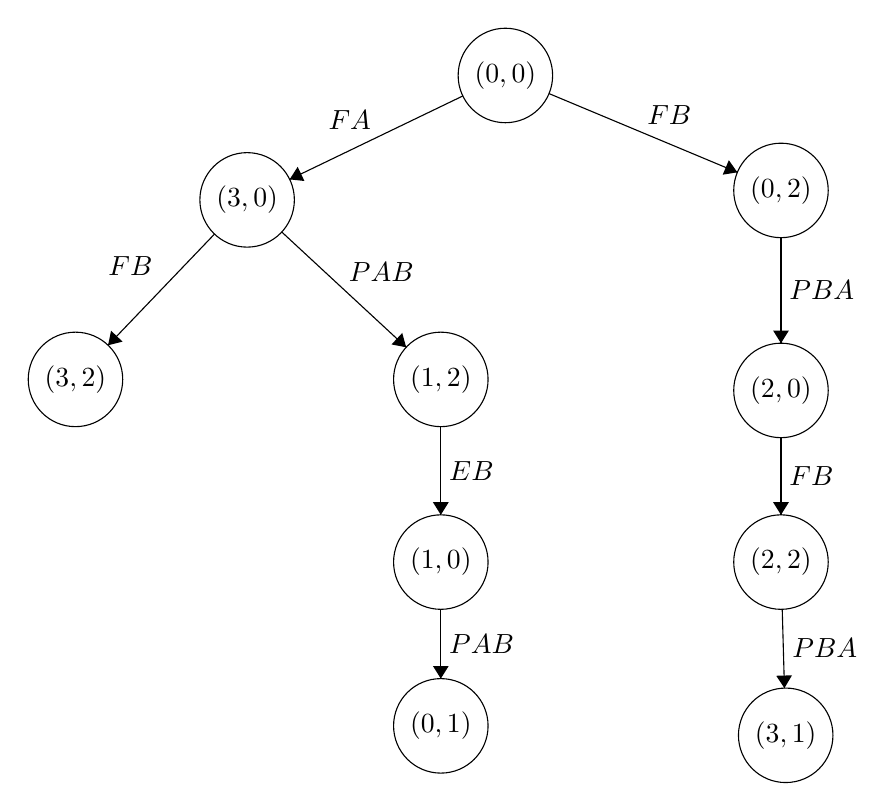
\begin{tikzpicture}[scale=0.2]
            \tikzstyle{every node}+=[inner sep=0pt]
            \draw [black] (38.4,-5.1) circle (3);
            \draw (38.4,-5.1) node {$(0,0)$};
            \draw [black] (22,-13) circle (3);
            \draw (22,-13) node {$(3,0)$};
            \draw [black] (55.9,-12.4) circle (3);
            \draw (55.9,-12.4) node {$(0,2)$};
            \draw [black] (11.1,-24.4) circle (3);
            \draw (11.1,-24.4) node {$(3,2)$};
            \draw [black] (34.3,-24.4) circle (3);
            \draw (34.3,-24.4) node {$(1,2)$};
            \draw [black] (55.9,-25.1) circle (3);
            \draw (55.9,-25.1) node {$(2,0)$};
            \draw [black] (34.3,-36) circle (3);
            \draw (34.3,-36) node {$(1,0)$};
            \draw [black] (55.9,-36) circle (3);
            \draw (55.9,-36) node {$(2,2)$};
            \draw [black] (34.3,-46.4) circle (3);
            \draw (34.3,-46.4) node {$(0,1)$};
            \draw [black] (56.2,-47) circle (3);
            \draw (56.2,-47) node {$(3,1)$};
            \draw [black] (35.7,-6.4) -- (24.7,-11.7);
            \fill [black] (24.7,-11.7) -- (25.64,-11.8) -- (25.21,-10.9);
            \draw (28.52,-8.54) node [above] {$FA$};
            \draw [black] (41.17,-6.25) -- (53.13,-11.25);
            \fill [black] (53.13,-11.25) -- (52.59,-10.48) -- (52.2,-11.4);
            \draw (48.81,-8.23) node [above] {$FB$};
            \draw [black] (19.93,-15.17) -- (13.17,-22.23);
            \fill [black] (13.17,-22.23) -- (14.09,-22) -- (13.36,-21.31);
            \draw (16.02,-17.23) node [left] {$FB$};
            \draw [black] (24.2,-15.04) -- (32.1,-22.36);
            \fill [black] (32.1,-22.36) -- (31.85,-21.45) -- (31.17,-22.18);
            \draw (30.52,-18.21) node [above] {$PAB$};
            \draw [black] (55.9,-15.4) -- (55.9,-22.1);
            \fill [black] (55.9,-22.1) -- (56.4,-21.3) -- (55.4,-21.3);
            \draw (56.4,-18.75) node [right] {$PBA$};
            \draw [black] (34.3,-27.4) -- (34.3,-33);
            \fill [black] (34.3,-33) -- (34.8,-32.2) -- (33.8,-32.2);
            \draw (34.8,-30.2) node [right] {$EB$};
            \draw [black] (55.9,-28.1) -- (55.9,-33);
            \fill [black] (55.9,-33) -- (56.4,-32.2) -- (55.4,-32.2);
            \draw (56.4,-30.55) node [right] {$FB$};
            \draw [black] (34.3,-39) -- (34.3,-43.4);
            \fill [black] (34.3,-43.4) -- (34.8,-42.6) -- (33.8,-42.6);
            \draw (34.8,-41.2) node [right] {$PAB$};
            \draw [black] (55.98,-39) -- (56.12,-44);
            \fill [black] (56.12,-44) -- (56.6,-43.19) -- (55.6,-43.22);
            \draw (56.59,-41.49) node [right] {$PBA$};
            \end{tikzpicture}
            \end{center}
	% part b
	\item Suppose we already construct the graph $T(V,E)$, then \proc{BucketMeasure}$(m, n, k)$ works as follow,
		\begin{itemize}
		\item First do a special case BFS on  tree $T(V, E)$ starts at root $(0,0)$, search for $k$ and return the first node $O(x,y)$ such that  $x = k$ or $y=k$. Return \proc{nil} if no such node exist.
		\item If BFS returns a node $O$ instead of \proc{nil}, then we do:
			
			\begin{itemize}[label = {}]
			\item$result = stack()$ 
			\item return  \proc{exactInfo}(O, result)
			\item 
			\item \proc{exactInfo}(node, stack):
				\begin{itemize}[label = {}]
				\item  if $node.parent \neq \proc{nil}$: 
				\item \ \ \ \ \ \ \ \ $list \leftarrow append(node.edgeInfo)$
				\item \ \ \ \ \ \ \ \ $\proc{exactInfo}(node.parent, stack)$
				\item return $list$
				\end{itemize}
			
			\end{itemize}
		
		\end {itemize}
	% proof of correctness
	Claim: \proc{BucketMeasure}$(m, n, k)$ returns a sequence of moves that results in one bucket (it does not matter which one) having exactly $k$ litres of water. The number of moves in the returned sequence is smallest.
		
		\begin{itemize}[label={}]
		\item Proof of Termination
		\item We know that BFS always terminates. It's clearly that  \proc{exactInfo} also always terminates if the input node is not  \proc{nil}, since the height of tree is finite. Therefore, proc{BucketMeasure}$(m, n, k)$ also terminates.
		\item
		\item Proof of Partial Correcness
		\item We know from the lecture that for BFS when search for $k$ it always returns the shortest the path from root to any node $(x,y)$ where  $x = k$ or $y=k$. Hence, we just need to proof $result$ contains the correct sequence of operations.
		\item This is also clear since we know stack always append to the top. Then when we trace back from the accepting state, the last operation is in the bottom the stack and the first operation is at top. Hence in correct sequence.
		\end{itemize}	
	% worst case run time 
	\item  \proc{Note:} The number of nodes and edges of tree we constructed from (a) are both in $\mathcal{O}{mn}$.
		\begin{itemize}[label={}]
		\item First a new states is added to the tree only if it is different from all previous states; hence, every node in the tree is unique. Then there are at most $(m+1)(n+1)$ combinations for states, which means the number of nodes  of tree is in $\mathcal{O}{mn}$.
		\item Secondly, we know that for three $|E| = |V| - 1$; therefore,  the number of edges  of tree is also in $\mathcal{O}{mn}$.
		\end{itemize}
		The worst case occurs when such $k$ does not exist, which means we have search every node in tree. Then the worst-case runtime is $\mathcal{O}{(mn)}$.
	\end{enumerate}	
\end{enumerate}

\end{document}
